\documentclass[]{book}

%These tell TeX which packages to use.
\usepackage{array,epsfig}
\usepackage{amsmath}
\usepackage{amsfonts}
\usepackage{amssymb}
\usepackage{amsxtra}
\usepackage{amsthm}
\usepackage{mathrsfs}
\usepackage{color}
\usepackage{multirow}
\usepackage{pgfplots}
\usepackage{hyperref}


%Here I define some theorem styles and shortcut commands for symbols I use often
\theoremstyle{definition}
\newtheorem{defn}{Definition}
\newtheorem{thm}{Theorem}
\newtheorem{cor}{Corollary}
\newtheorem*{rmk}{Remark}
\newtheorem{lem}{Lemma}
\newtheorem*{joke}{Joke}
\newtheorem{ex}{Example}
\newtheorem*{soln}{Solution}
\newtheorem{prop}{Proposition}

\newcommand{\lra}{\longrightarrow}
\newcommand{\ra}{\rightarrow}
\newcommand{\surj}{\twoheadrightarrow}
\newcommand{\graph}{\mathrm{graph}}
\newcommand{\bb}[1]{\mathbb{#1}}
\newcommand{\Z}{\bb{Z}}
\newcommand{\Q}{\bb{Q}}
\newcommand{\R}{\bb{R}}
\newcommand{\C}{\bb{C}}
\newcommand{\N}{\bb{N}}
\newcommand{\M}{\mathbf{M}}
\newcommand{\m}{\mathbf{m}}
\newcommand{\MM}{\mathscr{M}}
\newcommand{\HH}{\mathscr{H}}
\newcommand{\Om}{\Omega}
\newcommand{\Ho}{\in\HH(\Om)}
\newcommand{\bd}{\partial}
\newcommand{\del}{\partial}
\newcommand{\bardel}{\overline\partial}
\newcommand{\textdf}[1]{\textbf{\textsf{#1}}\index{#1}}
\newcommand{\img}{\mathrm{img}}
\newcommand{\ip}[2]{\left\langle{#1},{#2}\right\rangle}
\newcommand{\inter}[1]{\mathrm{int}{#1}}
\newcommand{\exter}[1]{\mathrm{ext}{#1}}
\newcommand{\cl}[1]{\mathrm{cl}{#1}}
\newcommand{\ds}{\displaystyle}
\newcommand{\vol}{\mathrm{vol}}
\newcommand{\cnt}{\mathrm{ct}}
\newcommand{\osc}{\mathrm{osc}}
\newcommand{\LL}{\mathbf{L}}
\newcommand{\UU}{\mathbf{U}}
\newcommand{\support}{\mathrm{support}}
\newcommand{\AND}{\;\wedge\;}
\newcommand{\OR}{\;\vee\;}
\newcommand{\Oset}{\varnothing}
\newcommand{\st}{\ni}
\newcommand{\wh}{\widehat}
\newcommand{\rank}[1]{\textrm{rank}({#1})}
\newcommand\yellow[1]{\colorbox{yellow}{#1}}
\newcommand\pink[1]{\colorbox{pink}{#1}}
\newcommand\ans{\underline{Answer}: }

%Pagination stuff.
\setlength{\topmargin}{-.3 in}
\setlength{\oddsidemargin}{0in}
\setlength{\evensidemargin}{0in}
\setlength{\textheight}{9.in}
\setlength{\textwidth}{6.5in}
\pagestyle{empty}



\begin{document}


\begin{center}
\textbf{Final test answers (Wednesday 14 December 2022, 15:00 CET)}\\ %You should put your name here
Elements of Mathematics -- Bioinformatics for Health Sciences \\
\end{center}

\vspace{0.2 cm}

\begin{enumerate}


% ----1----

\item {\bf (1 point)} Compute the inverse of the following matrix using Gauss-Jordan elimination:

\[
   M=
  \left[ {\begin{array}{ccc}
  1 & 0 & 0 \\
  -1 & 1 & 0 \\
  0 & 1 & 1
  \end{array} } \right].
\]

\ans Let's set up the block matrix with $M$ as top block and $\textrm{Id}$ as bottom block and apply elementary column operations until the top block is the identity matrix and (consequently) the bottom block (yellow) block is the inverse of M:

\[
{\begin{bmatrix}
1 & 0 & 0 \\
-1 & 1 & 0 \\ 
 0 & 1 & 1 \\
\yellow{1} & \yellow{0} & \yellow{0} \\
\yellow{0} &\yellow{1} &\yellow{0}  \\
\yellow{0}  & \yellow{0} & \yellow{1} 
  \end{bmatrix}
}
\stackrel{a}{\sim}
{\begin{bmatrix}
1 & 0 & 0   \\
-1 & 1 & 0   \\
 0 & 0 & 1 \\ 
\yellow{1} & \yellow{0} & \yellow{0} \\
\yellow{0} &\yellow{1} &\yellow{0} \\
\yellow{0}  & \yellow{-1} & \yellow{1} 
  \end{bmatrix}
}
\stackrel{b}{\sim}
{\begin{bmatrix}
1 & 0 & 0 \\
 0 & 1 & 0 \\
 0 & 0 & 1 \\
\yellow{1} & \yellow{0} & \yellow{0} \\
\yellow{1} &\yellow{1} &\yellow{0} \\
\yellow{-1}  & \yellow{-1} & \yellow{1} 
\end{bmatrix}},
\]

with steps: 
\begin{enumerate}
\item $C_2 \leftarrow C_2 - C_3$
\item $C_1 \leftarrow C_1 + C_2$
\end{enumerate}


% ----2----

\item Consider the following $3\times 3$ matrix:

\[
   A=
  \left[ {\begin{array}{ccc}
   -2 & 1 & -1 \\
   2 & -1 & 1 \\
   2 & -1 & 1 \\
  \end{array} } \right].
\]

\begin{enumerate}
\item {\bf (0.5 points)} What is the rank of the matrix A? Justify your answer.

\ans $\rank{A} = 1$ because all the column vectors are multiples of the vector $(1, -1, -1)$.

\item {\bf (0.5 points)} Write $A$ as the product of two matrices $U$ and $V$ with sizes $3\times 1$ and $1\times 3$, respectively.

\ans There are infinitely many solutions. We could take the following matrices:

\[
   U=
  \left[ 
  {\begin{array}{ccc}
  1 \\
  -1 \\
  -1 \\
  \end{array} } \right]
\;\;\;
   V=
  \left[
  {\begin{array}{ccc}
  -2 & 1 & -1 \\
  \end{array} } 
   \right]
\]

\end{enumerate} 




% ----3----


\item {\bf (1 point)} The \emph{index} of a matrix $A$ is defined as the dimension of its nullspace minus the dimension of the nullspace of $A^t$, i.e., $\dim{N(A)} - \dim{N(A^t)}$. If $A$ is a $7\times 9$ matrix of rank $5$, what is its index?

\ans

First observe that $\rank{A} = \rank{A^t}=5$.
Let's write down the fundamental theorem of linear algebra for both matrices $A$ and $A^t$:
\[
9 = \dim{N(A)} + \rank{A} \Rightarrow \dim{N(A)} = 9 - 5 = 4
\]
\[
7 = \dim{N(A^t)} + \rank{A^t} \Rightarrow \dim{N(A^t)} = 7 - 5 = 2
\]

The index of $A$ is $\dim{N(A)} - \dim{N(A^t)} = 4 - 2 = 2$.


% ----4----

\item This problem is about all possible solutions of $x + 2y + 2z + w = 0$, which can be regarded as a vector subspace of $\mathbb{R}^4$ given as the null space $N(A)$ of the matrix $A = \left[1\; 2\; 2\; 1\right]\in\mathbb{R}^{1\times 4}$. 


\begin{enumerate}

\item {\bf (1 point)} Give a basis of $N(A)$.

\ans

Applying Gauss-Jordan we see that:

\[
{\begin{bmatrix}
1 & 2 & 2 & 1\\
1 & \yellow{0} & \yellow{0} & \yellow{0} \\
0 &\yellow{1} &\yellow{0} &  \yellow{0} \\
0  & \yellow{0} & \yellow{1} &  \yellow{0} \\
0  & \yellow{0} & \yellow{0} &  \yellow{1} \\
  \end{bmatrix}
}
\stackrel{a,b,c}{\sim}
{\begin{bmatrix}
1 & 0 & 0 & 0 \\
1 & \yellow{-2} & \yellow{-2} & \yellow{-1} \\
0 &\yellow{1} &\yellow{0} &  \yellow{0} \\
0  & \yellow{0} & \yellow{1} &  \yellow{0} \\
0  & \yellow{0} & \yellow{0} &  \yellow{1} \\
  \end{bmatrix}
}
\]
 
using elementary column operations: 
\begin{enumerate}
\item[(a)] $C_2 \leftarrow C_2 - 2C_1$
\item[(b)] $C_3 \leftarrow C_3 - 2C_1$
\item[(c)] $C_4 \leftarrow C_4 - C_1$
\end{enumerate}

The vectors $u=(-2,1,0,0)$, $v=(-2,0,1,0)$ and $w=(-1,0,0,1)$ form a basis of $N(A)$.


\item {\bf (1 point)} Give an orthonormal basis of $N(A)$.

\ans (with option 1: using Gauss-Jordan elimination)

Let $A=[u|\; v\; w]$ then we conduct Gauss-Jordan elimination on the block matrix with $A^tA$ as the top block and $A$ as the bottom block.

\[
{\begin{bmatrix}
5 & 4 & 2\\
4 & 5 & 2 \\
2 & 2 & 2 \\

-2 & -2 & -1\\
1 & 0 & 0 \\
0 & 1 & 0 \\
0 & 0 & 1 \\
\end{bmatrix}
}
\stackrel{a,b}{\sim}
{\begin{bmatrix}
5 & 0 & 0\\
4 & 5 - \frac{4}{5}\cdot4 & 2 - \frac{2}{5}\cdot4 \\
2 & 2 - \frac{4}{5}\cdot2 & 2 - \frac{2}{5}\cdot2 \\

-2 & -2 + \frac{4}{5}\cdot2  & -1 + \frac{2}{5}\cdot2 \\
1 & -\frac{4}{5} & -\frac{2}{5} \\
0 & 1 & 0 \\
0 & 0 & 1 \\
\end{bmatrix}
}
=
{\begin{bmatrix}
5 & 0 & 0\\
4 & \frac{9}{5} & \frac{2}{5} \\
2 & \frac{2}{5} & \frac{6}{5} \\

-2 & -\frac{2}{5} & -\frac{1}{5}\\
1 & -\frac{4}{5} & -\frac{2}{5} \\
0 & 1 & 0 \\
0 & 0 & 1 \\
\end{bmatrix}
\stackrel{c}{\sim}
}
\]
\[
\stackrel{c}{\sim}
{\begin{bmatrix}
5 & 0 & 0\\
4 & \frac{9}{5} & 0 \\
2 & \frac{2}{5} & \frac{6}{5} - \frac{2}{9}\cdot\frac{2}{5} \\

-2 & -\frac{2}{5} & -\frac{1}{5} + \frac{2}{9}\cdot\frac{2}{5} \\
1 & -\frac{4}{5} & -\frac{2}{5} +\frac{2}{9}\cdot\frac{4}{5} \\
0 & 1 & -\frac{2}{9} \\
0 & 0 & 1 \\
\end{bmatrix}
}
=
{\begin{bmatrix}
5 & 0 & 0\\
4 & \frac{9}{5} & 0 \\
2 & \frac{2}{5} & \frac{10}{9} \\

-2 & -\frac{2}{5} & -\frac{1}{9} \\
1 & -\frac{4}{5} & -\frac{2}{9} \\
0 & 1 & -\frac{2}{9} \\
0 & 0 & 1 \\
\end{bmatrix}
}
\]

we get column echellon matrix in the top block using the elementary column operations: 
\begin{enumerate}
\item[(a)] $C_2 \leftarrow C_2 - \frac{4}{5}C_1$
\item[(b)] $C_3 \leftarrow C_3 - \frac{2}{5}C_1$
\item[(c)] $C_3 \leftarrow C_2 - \frac{2}{9}C_2$
\end{enumerate}

This solution -- the column vectors of the bottom block -- provides an orthogonal basis of $\textrm{span}\{u,v,w\}$  that can be subsequently transformed into an orthonormal basis just by dividing each vector by its length:

\[
\tilde{u} = \frac{1}{\sqrt{5}}(-2,1,0,0)
\]
\[
\tilde{v} = \frac{1}{\sqrt{4+16+25}}(-2,-4,5,0) = \frac{1}{3\sqrt{5}}(-2,-4,5,0)
\]
\[
\tilde{w} = \frac{1}{\sqrt{1+4+4+81}}(-1,-2,-2,9) = \frac{1}{3\sqrt{10}}(-1,-2,-2,9)
\]



\ans (with option 2: iterative procedure)

We can obtain the result by applying the Gram-Schmidt method. This method constructs an orthonormal basis of $\textrm{span}\{u,v,w\}$ by recurrently adding rectified versions of the vectors with respect to the orthornormal subset that has already been created. More concretely:

We start by re-scaling $u$ to have length 1:
\[
\tilde{u} = \frac{u}{\| u \|} = \frac{1}{\sqrt{5}}(-2,1,0,0).
\]


Then we must produce a rectified version of $v$, so that the resulting vector is orthogonal to $\tilde{u}$ and has length 1. In order to accomplish orthogonality, we simply remove from $v$ its orthogonal projection onto $\textrm{span}\{u\}$:
\[
\tilde{v}_0 = v - (v\cdot \tilde{u})\tilde{u} = (-2,0,1,0) - \frac{4}{\sqrt{5}} \frac{1}{\sqrt{5}} (-2,1,0,0) = (-2/5, -4/5, 1, 0)
\]
\[
\|\tilde{v}_0\| = \frac{1}{5} \sqrt{4 + 16 + 25} = \frac{1}{5}\sqrt{45} = \frac{3}{5}\sqrt{5}
\]
\[
\tilde{v} = \tilde{v}_0 / \| \tilde{v}_0 \| = \frac{1}{3\sqrt{5}} (-2,-4,5,0)
\]


Now $\{\tilde{u}, \tilde{v}\}$ is an orthonormal subset that spans the same vector subspace as $\{u,v\}$. We must compute now a rectified version of $w$, so that the resulting vector is orthogonal to $\textrm{span}\{u,v\}$ and has length 1. In order to accomplish orthogonality, we simply remove from $w$ its orthogonal projection onto $\textrm{span}\{\tilde{u}, \tilde{v}\}$:
\[
\tilde{w}_0 = w - (w\cdot \tilde{u})\tilde{u} - (w\cdot \tilde{v})\tilde{v}
\]
\[
(w\cdot \tilde{u})\tilde{u} = \frac{2}{\sqrt{5}}\frac{1}{\sqrt{5}}(-2,1,0,0) = (-4/5, 2/5, 0, 0)
\]
\[
(w\cdot \tilde{v})\tilde{v} =  \frac{2}{3\sqrt{5}}\frac{1}{3\sqrt{5}}(-2,-4,5,0) = (-4/45, -8/45, 10/45, 0)
\]

\[
\tilde{w}_0 = w - (w\cdot \tilde{u})\tilde{u} - (w\cdot \tilde{v})\tilde{v} = (-1, 0, 0, 1) - (-4/5, 2/5, 0, 0) - (-4/45, -8/45, 10/45, 0) =
\]
\[
= (-1 + 4/5 + 4/45, -2/5 + 8/45, -10/45, 1) = (-1/9, -2/9, -2/9, 1)
\]
\[
\tilde{w} = \tilde{w}_0 / \| \tilde{w}_0 \| = \frac{1}{3\sqrt{10}} (-1, -2, -2, 9)
\]



\end{enumerate}


%----5----

\item In this exercise we will study the so-called \emph{softplus} function:
\[
f_k(x) = \frac{1}{k}\log(1+e^{kx})
\]
where $k>0$ is a parameter, known as \emph{sharpness}.

\begin{enumerate}

\item {\bf(0.5 points)} Compute the first derivative of $f_k(x)$. What are its values at $x=0$ and $x=-1$, respectively?

\ans
Applying the chain rule:
\[
f'_k(x) =\frac{1}{k} \cdot \frac{1}{1+e^{kx}} \cdot ke^{kx}  = \frac{e^{kx}}{1+e^{kx}} = \frac{1}{1 + e^{-kx}}
\]
\[
f'_k(0) = \frac{1}{2} \;\; \textrm{and} \;\; f'_k(-1) = \frac{1}{1+e^{k}}
\]

\item {\bf (1 point)} Compute the Taylor approximation of $f_k$ of order 2 at $x=0$.

\ans

The Taylor approximation has this form:
\[
T_k(x) = f_k(0) + f'_k(0)x + \frac{1}{2}f''_k(0)x^2 + o(x^2)
\]
Let's compute and evaluate the function and its first and second derivatives at $x=0$:
\[
f_k(0) = \frac{\log 2}{k}
\]
\[
f'_k(x) = (1 + e^{-kx})^{-1} \Rightarrow f'_k(0) = \frac{1}{2}
\]

Let's compute the second derivative by applying the chain rule on first derivative:

\[
f''_k(x) = ((1 + e^{-kx})^{-1})' = -(1+e^{-kx})^{-2}\cdot (-k)e^{-kx} = \frac{ke^{-kx}}{(1 + e^{-kx})^2} \Rightarrow f''_k(0) = \frac{k}{4} 
\]
The sought Taylor approximation is:
\[
T_k(x) = \frac{\log 2}{k} + \frac{1}{2}x + \frac{k}{8}x^2 + o(x^2)
\]

\item {\bf (0.5 points)} Explain why you think the parameter $k$ is known as \emph{sharpness}. It may be helpful to sketch the graph of the function -- using all the information you have -- for different values of $k$.

\ans

There are several hints that can be used. Note that the function is positive everywhere. Also note that the intercept $f_k(0)=\log2 / k$ gets smaller with increasing values of $k$, but the slope of the graph at $x=0$ is $1/2$ regardless of the value of $k$. You also may observe that the derivative of the function is always $>0$, so the function is increasing everywhere and has no critical points. What all this information indicates is that the graph of the function must have an "elbow" below $x=0$ that gets sharper (!) with larger values of $k$. For $k\to\infty$ this function approximates the rectified linear unit $\textrm{ReLU}(x) = \max\{0, x\}$

\begin{center}
\begin{tikzpicture}
  \begin{axis} [axis lines=center]
    \addplot [blue!15, domain=-2:0.7, smooth, thick] {ln(1 + e^(\x))} node[black!100, pos=0.94] {$k=1$};
    \addplot [blue!55, domain=-2:0.7, smooth, thick] {1/10*ln(1 + e^(10*\x))} node[black!100, pos=0.85] {$k=10$};
  \end{axis}
\end{tikzpicture}
\end{center}


\end{enumerate}



% ----6----

\item In this exercise we are going to study the critical points of the function
\[
f(x, y) = x^2 - xy + y^3.
\]

\begin{enumerate}

\item {\bf (1 point)}  Compute the critical points of $f$.

\ans

Let's compute the first partial derivatives:

\[
\frac{\partial f}{\partial x} =  2x - y, \;\;\; \frac{\partial f}{\partial y} =  -x + 3y^2
\]

The critical points are those where both partial derivatives vanish, i.e., the points satisfying the two equations $2x = y$ and $3y^2 = x$. Substituting $y$ in the second equation we get $12x^2 - x = 0$, which in turn leaves us with two possibilities: $x = 0$ and $x=1/12$. Hence $f$ has two critical points: $P_0 = (0,0)$ and $P_1=(1/12, 1/6)$.

\item {\bf (2 points)}  Compute the eigenvalues of the Hessian matrices at the critical points and determine whether the critical points are local maxima, local minima or saddle points.

\ans

To assert the nature of the critical points, we need to compute the Hessian matrix of $f$. Let's start by computing the second order partial derivatives of $f$:

\[
\frac{\partial^2 f}{\partial x^2} =  2, \;\;\; \frac{\partial^2 f}{\partial y^2} =  6y, \;\;\; \frac{\partial^2 f}{\partial x \partial y} = -1
\]

The general form of the Hessian matrix of $f$ is: 

\[
Hf(x,y) = \begin{bmatrix}
2 & -1 \\
-1 & 6y
\end{bmatrix}
\]

\vspace{1cm}

\underline{Hessian matrix at $P_0 = (0,0)$}

\[
H_0 = Hf(P_0) = \begin{bmatrix}
2 & -1 \\
-1 & 0
\end{bmatrix}
\]

The characteristic polynomial of $H_0$ is 
\[
Q_0(t) = t(t-2)-1.
\] 
Here you can apply the formula for solving quadratic equations with one variable. Alternatively, you use the technique known as \href{https://en.wikipedia.org/wiki/Completing_the_square}{completing the square} alongside the well-known identity $a^2 - b^2 = (a+b)(a-b)$ to factor our degree 2 characteristic polynomials, thereby finding its roots. I will be using this technique to illustrate how it works in practice. 

Back to our characteristic polynomial:
\[
Q_0(t) = t(t-2)-1 = t^2 - 2t - 1 = (t+1)^2 - 2 = (t+1+\sqrt{2})(t+1-\sqrt{2}),
\] 

with roots $\lambda_1 = -1-\sqrt{2}<0$ and $\lambda_2 = -1+\sqrt{2}>0$. Since the eigenvalues have opposite signs, $P_0$ is a saddle point. 

\vspace{1cm}

\underline{The Hessian matrix at $P_1 = (1/12, 1/6)$}

\[
H_1 = Hf(P_1) = \begin{bmatrix}
2 & -1 \\
-1 & 1
\end{bmatrix}
\]

The characteristic polynomial of $H_1$ is 
\[
Q_1(t) =(t-1)(t-2)-1 = t^2 - 3t +1 = (t - 3/2)^2 - 5/4 = (t - 3/2 + \sqrt{5}/2)(t - 3/2 - \sqrt{5}/2)
\]
with roots $\lambda_1 = (3 - \sqrt{5})/2 > 0$ and $\lambda_2=(3 + \sqrt{5})/2 > 0$. In particular, we can see that the two eigenvalues are positive, hence $P_1$ is a local minimum.

\end{enumerate}




\end{enumerate}

\end{document}


